\documentclass[border=6pt]{standalone}
\usepackage{tikz}
\usepackage{pgfplots}
\pgfplotsset{compat=1.18}
\usetikzlibrary{arrows.meta,positioning,shapes.geometric,fit,backgrounds,calc,decorations.pathreplacing,patterns,pgfplots.groupplots}
\tikzset{
  blk/.style={rectangle, rounded corners=2pt, draw=black!70, thick, fill=blue!6,
              minimum height=8mm, minimum width=20mm, align=center, font=\small},
  io/.style={rectangle, rounded corners=6pt, draw=black!70, thick, fill=green!8,
             minimum height=8mm, align=center, font=\small},
  proc/.style={rectangle, draw=black!70, thick, fill=orange!10, minimum height=8mm,
               align=center, font=\small},
  dec/.style={diamond, aspect=2, draw=black!70, thick, fill=yellow!15, align=center, font=\footnotesize},
  warnbox/.style={rectangle, rounded corners=2pt, draw=red!60!black, thick, fill=red!7,
                  minimum height=8mm, align=center, font=\small},
  oklbox/.style={rectangle, rounded corners=2pt, draw=green!45!black, thick, fill=green!8,
                 minimum height=8mm, align=center, font=\small},
  ar/.style={-{Latex[length=2mm]}, thick},
  arl/.style={-{Latex[length=2mm]}, thick, dashed, draw=black!55},
  lbl/.style={font=\footnotesize\itshape, text=black!60},
}
\definecolor{good}{RGB}{34,139,34}
\definecolor{bad}{RGB}{178,34,34}
\definecolor{warn}{RGB}{218,165,32}
\definecolor{pesblue}{RGB}{0,45,98}
\definecolor{complete}{RGB}{30,125,79}
\definecolor{partial}{RGB}{176,106,0}
\definecolor{blocked}{RGB}{166,43,43}
\begin{document}
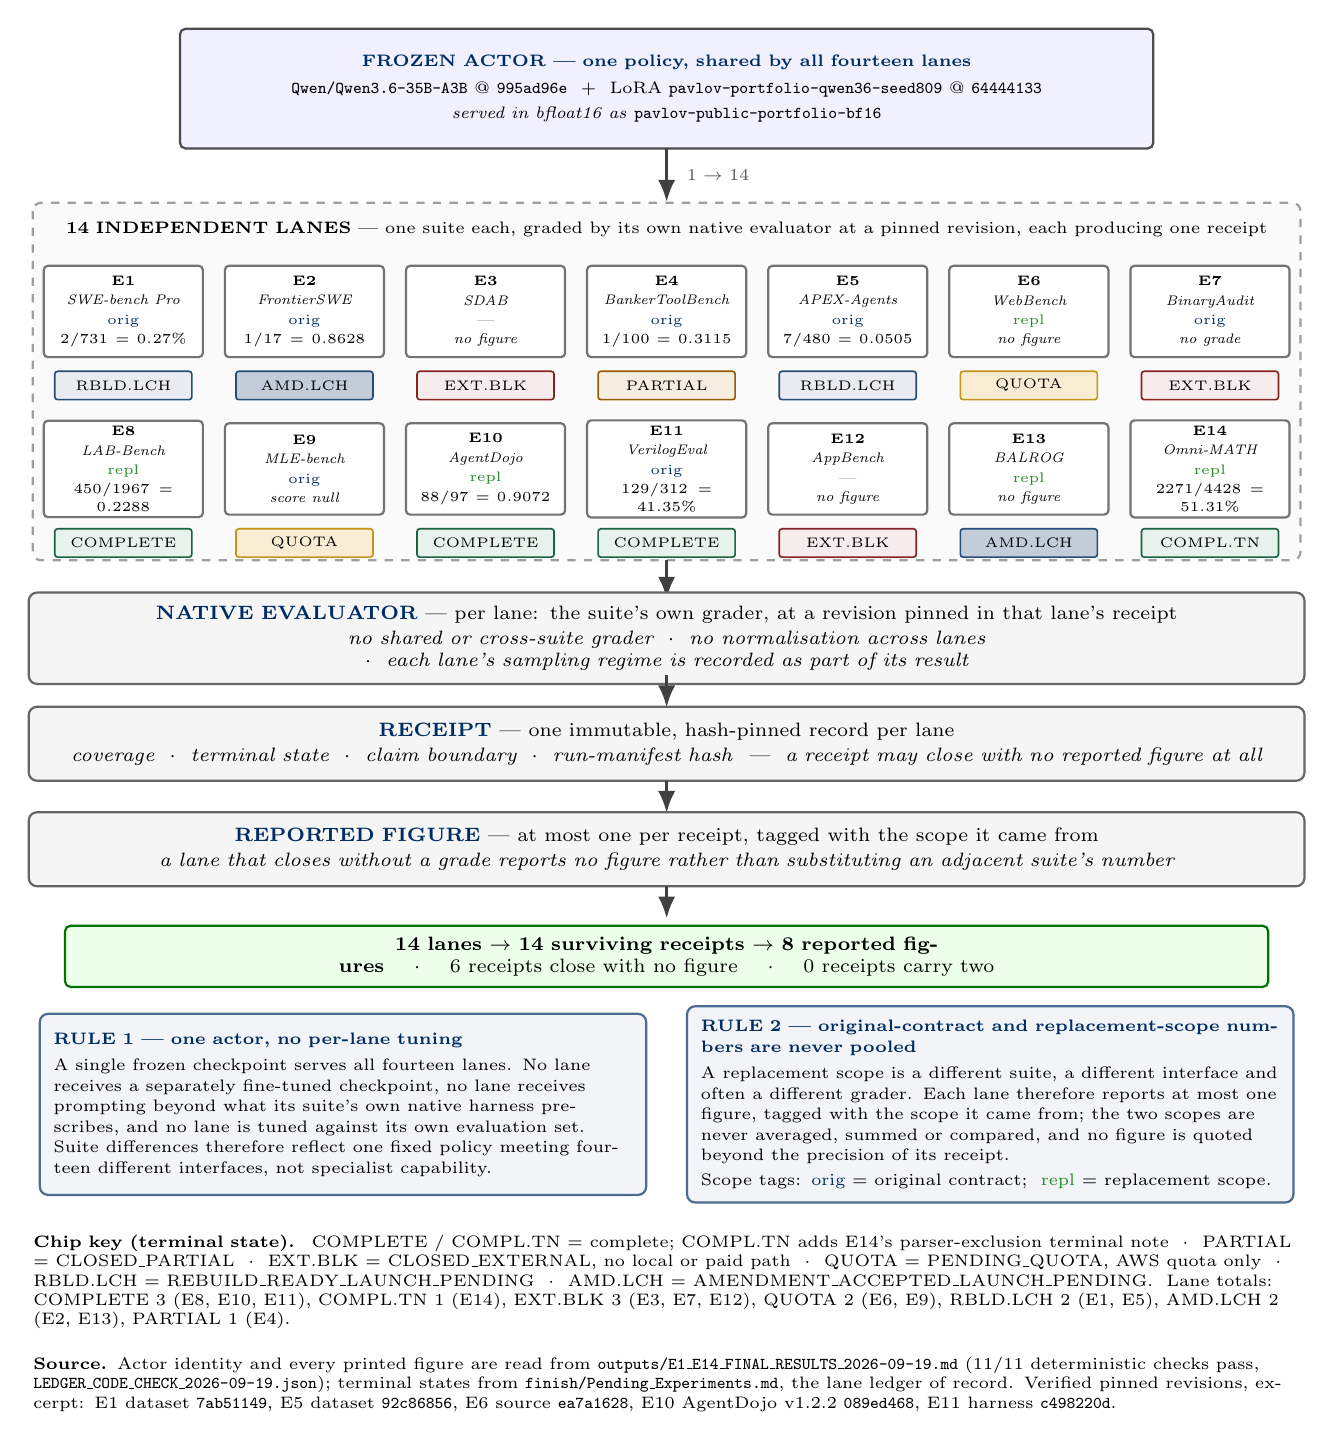
\begin{tikzpicture}[x=1cm,y=1cm,
  lane/.style={rectangle, rounded corners=1.5pt, draw=black!55, thick, fill=white,
               font={\fontsize{5.3}{6.4}\selectfont}, align=center,
               text width=1.88cm, inner sep=2pt, minimum height=1.16cm},
  chip/.style={rectangle, rounded corners=1pt, semithick, align=center,
               font={\fontsize{4.8}{5.5}\selectfont}, inner sep=1.5pt,
               minimum width=1.74cm, minimum height=0.36cm},
  chipC/.style={chip, draw=complete!80!black,  fill=complete!10},
  chipP/.style={chip, draw=partial!85!black,   fill=partial!12},
  chipB/.style={chip, draw=blocked!80!black,   fill=blocked!9},
  chipQ/.style={chip, draw=warn!90!black,      fill=warn!20},
  chipR/.style={chip, draw=pesblue!85,         fill=pesblue!9},
  chipA/.style={chip, draw=pesblue!85,         fill=pesblue!24},
  rail/.style={rectangle, rounded corners=3pt, draw=black!60, thick, fill=black!4,
               align=center, inner sep=5pt, text width=15.85cm, minimum height=0.94cm,
               font={\fontsize{6.6}{7.8}\selectfont}},
  rulebox/.style={rectangle, rounded corners=3pt, draw=pesblue!70, thick, fill=pesblue!5,
                  align=left, inner sep=5pt, minimum height=2.30cm},
  sar/.style={-{Latex[length=2.8mm,width=2.2mm]}, line width=1.2pt, draw=black!75},
  fin/.style={font={\fontsize{5.8}{7.0}\selectfont}, align=left, text width=16.10cm,
              anchor=north west, inner sep=0pt},
]

% ------------------------------------------------------------------
% 1. FROZEN ACTOR
% ------------------------------------------------------------------
\node[blk, text width=12.15cm, minimum height=1.52cm, inner sep=3pt,
      font={\fontsize{6.4}{7.7}\selectfont}, align=center] (actor) at (8.05,0)
  {{\bfseries\color{pesblue}FROZEN ACTOR --- one policy, shared by all fourteen lanes}\\[2pt]
   \texttt{Qwen/Qwen3.6-35B-A3B} @ \texttt{995ad96e} \ $+$ \ LoRA
   \texttt{pavlov-portfolio-qwen36-seed809} @ \texttt{64444133}\\[1.5pt]
   \textit{served in bfloat16 as} \texttt{pavlov-public-portfolio-bf16}};

\draw[sar] (8.05,-0.76) -- (8.05,-1.44);
\node[font={\fontsize{6.0}{7.0}\selectfont\itshape}, text=black!65,
      anchor=west, inner sep=0pt] at (8.30,-1.10) {$1 \rightarrow 14$};

% ------------------------------------------------------------------
% 2. LANE BLOCK (background)
% ------------------------------------------------------------------
\fill[black!2, rounded corners=3pt] (0,-1.45) rectangle (16.10,-5.99);
\draw[black!38, dashed, thick, rounded corners=3pt] (0,-1.45) rectangle (16.10,-5.99);

\node[font={\fontsize{6.3}{7.4}\selectfont}, align=center, inner sep=0pt,
      text width=15.5cm] at (8.05,-1.79)
  {{\bfseries 14 INDEPENDENT LANES} --- one suite each, graded by its own native
   evaluator at a pinned revision, each producing one receipt};

% --- column x positions: 1.15 3.45 5.75 8.05 10.35 12.65 14.95 -------------
% --- row 1 (E1-E7) ---------------------------------------------------------
\node[lane] (L1) at (1.15,-2.83)
  {{\bfseries E1}\\[0.6pt]{\itshape SWE-bench Pro}\\[0.6pt]{\color{pesblue}orig}\\[0.6pt]$2/731 = 0.27\%$};
\node[chipR] (C1) at (1.15,-3.77) {RBLD.LCH};

\node[lane] (L2) at (3.45,-2.83)
  {{\bfseries E2}\\[0.6pt]{\itshape FrontierSWE}\\[0.6pt]{\color{pesblue}orig}\\[0.6pt]$1/17 = 0.8628$};
\node[chipA] (C2) at (3.45,-3.77) {AMD.LCH};

\node[lane] (L3) at (5.75,-2.83)
  {{\bfseries E3}\\[0.6pt]{\itshape SDAB}\\[0.6pt]{\color{black!45}---}\\[0.6pt]{\itshape no figure}};
\node[chipB] (C3) at (5.75,-3.77) {EXT.BLK};

\node[lane] (L4) at (8.05,-2.83)
  {{\bfseries E4}\\[0.6pt]{\itshape BankerToolBench}\\[0.6pt]{\color{pesblue}orig}\\[0.6pt]$1/100 = 0.3115$};
\node[chipP] (C4) at (8.05,-3.77) {PARTIAL};

\node[lane] (L5) at (10.35,-2.83)
  {{\bfseries E5}\\[0.6pt]{\itshape APEX-Agents}\\[0.6pt]{\color{pesblue}orig}\\[0.6pt]$7/480 = 0.0505$};
\node[chipR] (C5) at (10.35,-3.77) {RBLD.LCH};

\node[lane] (L6) at (12.65,-2.83)
  {{\bfseries E6}\\[0.6pt]{\itshape WebBench}\\[0.6pt]{\color{good}repl}\\[0.6pt]{\itshape no figure}};
\node[chipQ] (C6) at (12.65,-3.77) {QUOTA};

\node[lane] (L7) at (14.95,-2.83)
  {{\bfseries E7}\\[0.6pt]{\itshape BinaryAudit}\\[0.6pt]{\color{pesblue}orig}\\[0.6pt]{\itshape no grade}};
\node[chipB] (C7) at (14.95,-3.77) {EXT.BLK};

% --- row 2 (E8-E14) --------------------------------------------------------
\node[lane] (L8) at (1.15,-4.83)
  {{\bfseries E8}\\[0.6pt]{\itshape LAB-Bench}\\[0.6pt]{\color{good}repl}\\[0.6pt]$450/1967 = 0.2288$};
\node[chipC] (C8) at (1.15,-5.77) {COMPLETE};

\node[lane] (L9) at (3.45,-4.83)
  {{\bfseries E9}\\[0.6pt]{\itshape MLE-bench}\\[0.6pt]{\color{pesblue}orig}\\[0.6pt]{\itshape score null}};
\node[chipQ] (C9) at (3.45,-5.77) {QUOTA};

\node[lane] (L10) at (5.75,-4.83)
  {{\bfseries E10}\\[0.6pt]{\itshape AgentDojo}\\[0.6pt]{\color{good}repl}\\[0.6pt]$88/97 = 0.9072$};
\node[chipC] (C10) at (5.75,-5.77) {COMPLETE};

\node[lane] (L11) at (8.05,-4.83)
  {{\bfseries E11}\\[0.6pt]{\itshape VerilogEval}\\[0.6pt]{\color{pesblue}orig}\\[0.6pt]$129/312 = 41.35\%$};
\node[chipC] (C11) at (8.05,-5.77) {COMPLETE};

\node[lane] (L12) at (10.35,-4.83)
  {{\bfseries E12}\\[0.6pt]{\itshape AppBench}\\[0.6pt]{\color{black!45}---}\\[0.6pt]{\itshape no figure}};
\node[chipB] (C12) at (10.35,-5.77) {EXT.BLK};

\node[lane] (L13) at (12.65,-4.83)
  {{\bfseries E13}\\[0.6pt]{\itshape BALROG}\\[0.6pt]{\color{good}repl}\\[0.6pt]{\itshape no figure}};
\node[chipA] (C13) at (12.65,-5.77) {AMD.LCH};

\node[lane] (L14) at (14.95,-4.83)
  {{\bfseries E14}\\[0.6pt]{\itshape Omni-MATH}\\[0.6pt]{\color{good}repl}\\[0.6pt]$2271/4428 = 51.31\%$};
\node[chipC] (C14) at (14.95,-5.77) {COMPL.TN};

% ------------------------------------------------------------------
% 3. THREE GOVERNANCE RAILS
% ------------------------------------------------------------------
\draw[sar] (8.05,-5.99) -- (8.05,-6.48);

\node[rail] (R1) at (8.05,-6.98)
  {{\bfseries\color{pesblue}NATIVE EVALUATOR} --- per lane: the suite's own grader,
   at a revision pinned in that lane's receipt\\[1.2pt]
   {\itshape no shared or cross-suite grader \ $\cdot$ \ no normalisation across lanes
   \ $\cdot$ \ each lane's sampling regime is recorded as part of its result}};

\draw[sar] (8.05,-7.45) -- (8.05,-7.86);

\node[rail] (R2) at (8.05,-8.32)
  {{\bfseries\color{pesblue}RECEIPT} --- one immutable, hash-pinned record per lane\\[1.2pt]
   {\itshape coverage \ $\cdot$ \ terminal state \ $\cdot$ \ claim boundary \ $\cdot$ \
   run-manifest hash \ --- \ a receipt may close with no reported figure at all}};

\draw[sar] (8.05,-8.79) -- (8.05,-9.20);

\node[rail] (R3) at (8.05,-9.66)
  {{\bfseries\color{pesblue}REPORTED FIGURE} --- at most one per receipt, tagged with
   the scope it came from\\[1.2pt]
   {\itshape a lane that closes without a grade reports no figure rather than
   substituting an adjacent suite's number}};

\draw[sar] (8.05,-10.13) -- (8.05,-10.54);

\node[oklbox, text width=15.0cm, minimum height=0.62cm, inner sep=4pt,
      font={\fontsize{6.7}{7.9}\selectfont}, align=center] (tally) at (8.05,-11.02)
  {{\bfseries 14 lanes $\rightarrow$ 14 surviving receipts $\rightarrow$ 8 reported figures}
   \quad $\cdot$ \quad 6 receipts close with no figure \quad $\cdot$ \quad 0 receipts carry two};

% ------------------------------------------------------------------
% 4. THE TWO GOVERNING RULES
% ------------------------------------------------------------------
\node[rulebox, text width=7.35cm, inner sep=5pt,
      font={\fontsize{6.2}{7.4}\selectfont}, align=left] (rule1) at (3.94,-12.90)
  {{\bfseries\color{pesblue}RULE 1 --- one actor, no per-lane tuning}\\[2.2pt]
   A single frozen checkpoint serves all fourteen lanes. No lane receives a
   separately fine-tuned checkpoint, no lane receives prompting beyond what its
   suite's own native harness prescribes, and no lane is tuned against its own
   evaluation set. Suite differences therefore reflect one fixed policy meeting
   fourteen different interfaces, not specialist capability.};

\node[rulebox, text width=7.35cm, inner sep=5pt,
      font={\fontsize{6.2}{7.4}\selectfont}, align=left] (rule2) at (12.16,-12.90)
  {{\bfseries\color{pesblue}RULE 2 --- original-contract and replacement-scope numbers
   are never pooled}\\[2.2pt]
   A replacement scope is a different suite, a different interface and often a
   different grader. Each lane therefore reports at most one figure, tagged with
   the scope it came from; the two scopes are never averaged, summed or compared,
   and no figure is quoted beyond the precision of its receipt.\\[1.6pt]
   Scope tags: {\color{pesblue}orig} $=$ original contract; \
   {\color{good}repl} $=$ replacement scope.};

% ------------------------------------------------------------------
% 5. KEYS AND PROVENANCE
% ------------------------------------------------------------------
\node[fin] at (0,-14.55)
  {{\bfseries Chip key (terminal state).} \
   COMPLETE / COMPL.TN $=$ complete; COMPL.TN adds E14's parser-exclusion terminal
   note \ $\cdot$ \ PARTIAL $=$ CLOSED\_PARTIAL \ $\cdot$ \
   EXT.BLK $=$ CLOSED\_EXTERNAL, no local or paid path \ $\cdot$ \
   QUOTA $=$ PENDING\_QUOTA, AWS quota only \ $\cdot$ \
   RBLD.LCH $=$ REBUILD\_READY\_LAUNCH\_PENDING \ $\cdot$ \
   AMD.LCH $=$ AMENDMENT\_ACCEPTED\_LAUNCH\_PENDING. \ Lane totals: COMPLETE 3
   (E8, E10, E11), COMPL.TN 1 (E14), EXT.BLK 3 (E3, E7, E12), QUOTA 2 (E6, E9),
   RBLD.LCH 2 (E1, E5), AMD.LCH 2 (E2, E13), PARTIAL 1 (E4).};

\node[fin] at (0,-16.10)
  {{\bfseries Source.} Actor identity and every printed figure are read from
   \texttt{outputs/E1\_E14\_FINAL\_RESULTS\_2026-09-19.md} (11/11 deterministic
   checks pass, \texttt{LEDGER\_CODE\_CHECK\_2026-09-19.json}); terminal states from
   \texttt{finish/Pending\_Experiments.md}, the lane ledger of record.
   Verified pinned revisions, excerpt: E1 dataset \texttt{7ab51149}, E5 dataset
   \texttt{92c86856}, E6 source \texttt{ea7a1628}, E10 AgentDojo v1.2.2
   \texttt{089ed468}, E11 harness \texttt{c498220d}.};

\end{tikzpicture}
\end{document}
